% =====================================================================
% Method-evolution diagram for the PINN-pricing paper.
% Stand-alone document — compile with:
%   pdflatex architecture.tex
% Produces architecture.pdf, included in paper.qmd via:
%   ![Method evolution](figures/architecture.pdf){#fig-architecture}
% =====================================================================
\documentclass[border=10pt]{standalone}

\usepackage{tikz}
\usetikzlibrary{positioning, arrows.meta, fit, backgrounds, calc}

\begin{document}
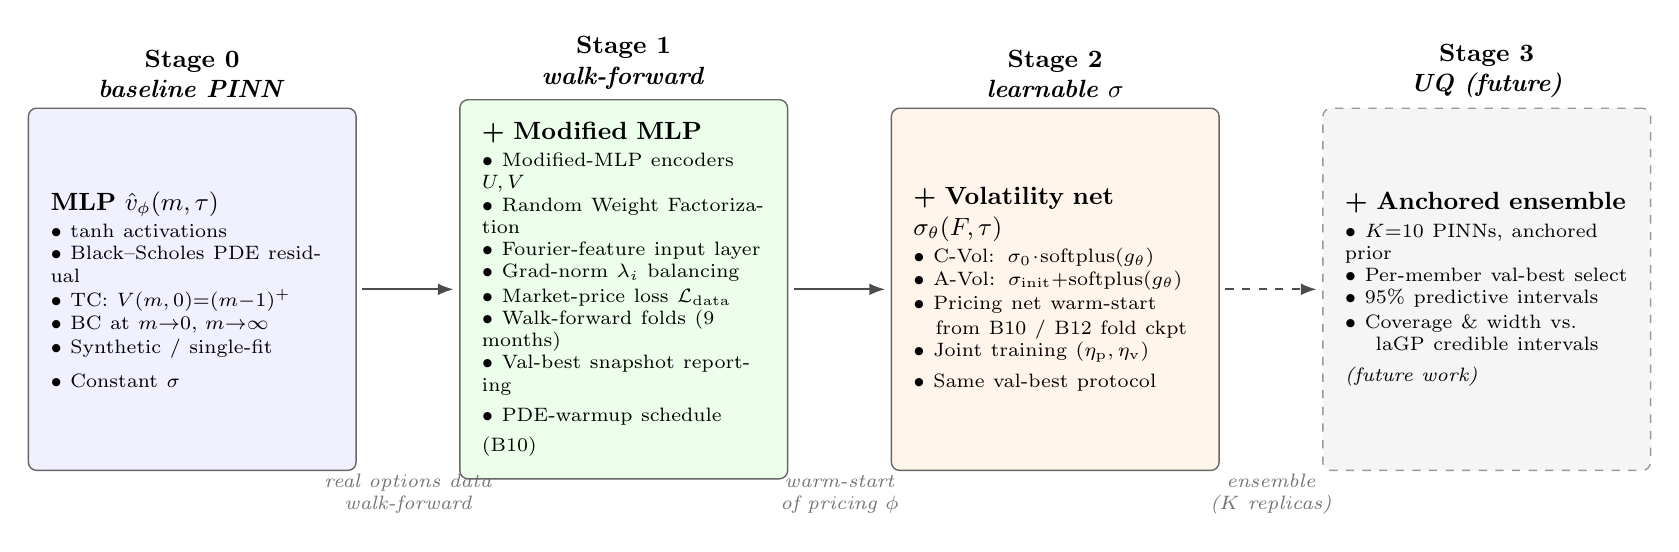
\begin{tikzpicture}[
    font=\small,
    stagebox/.style={
        draw=black!60, line width=0.5pt, rounded corners=3pt,
        align=left, inner sep=8pt, minimum width=4.0cm, minimum height=4.6cm,
        text width=3.6cm, fill=#1
    },
    titlebox/.style={
        font=\bfseries\small, anchor=south,
        align=center, text=black
    },
    addedlist/.style={
        align=left, anchor=north west, font=\scriptsize,
        text width=3.5cm
    },
    futurebox/.style={
        draw=black!40, line width=0.5pt, rounded corners=3pt, dashed,
        align=left, inner sep=8pt, minimum width=4.0cm, minimum height=4.6cm,
        text width=3.6cm, fill=gray!8
    },
    flowarrow/.style={
        -{Latex[length=2mm, width=1.5mm]},
        line width=0.7pt, draw=black!70, shorten >=2pt, shorten <=2pt
    }
]

% --- Stage 0 ---
\node[stagebox=blue!6] (s0) at (0, 0) {%
    \textbf{MLP $\hat v_\phi(m,\tau)$}\\[2pt]
    \scriptsize $\bullet$ $\tanh$ activations\\
    \scriptsize $\bullet$ Black--Scholes PDE residual\\[1pt]
    \scriptsize $\bullet$ TC: $V(m,0){=}(m{-}1)^+$\\
    \scriptsize $\bullet$ BC at $m{\to}0,\,m{\to}\infty$\\[1pt]
    \scriptsize $\bullet$ Synthetic / single-fit\\[1pt]
    \scriptsize $\bullet$ Constant $\sigma$
};
\node[titlebox] at (s0.north) {Stage 0 \\ \textit{baseline PINN}};

% --- Stage 1 ---
\node[stagebox=green!8, right=1.3cm of s0] (s1) {%
    \textbf{+ Modified MLP}\\[2pt]
    \scriptsize $\bullet$ Modified-MLP encoders $U,V$\\
    \scriptsize $\bullet$ Random Weight Factorization\\
    \scriptsize $\bullet$ Fourier-feature input layer\\
    \scriptsize $\bullet$ Grad-norm $\lambda_i$ balancing\\[1pt]
    \scriptsize $\bullet$ Market-price loss $\mathcal{L}_\mathrm{data}$\\
    \scriptsize $\bullet$ Walk-forward folds (9 months)\\
    \scriptsize $\bullet$ Val-best snapshot reporting\\
    \scriptsize $\bullet$ PDE-warmup schedule (B10)
};
\node[titlebox] at (s1.north) {Stage 1 \\ \textit{walk-forward}};

% --- Stage 2 ---
\node[stagebox=orange!8, right=1.3cm of s1] (s2) {%
    \textbf{+ Volatility net $\sigma_\theta(F,\tau)$}\\[2pt]
    \scriptsize $\bullet$ C-Vol: $\sigma_0\!\cdot\!\mathrm{softplus}(g_\theta)$\\
    \scriptsize $\bullet$ A-Vol: $\sigma_\mathrm{init}{+}\mathrm{softplus}(g_\theta)$\\[1pt]
    \scriptsize $\bullet$ Pricing net warm-start\\[1pt]
    \scriptsize $\quad$from B10 / B12 fold ckpt\\
    \scriptsize $\bullet$ Joint training $(\eta_\mathrm{p},\eta_\mathrm{v})$\\
    \scriptsize $\bullet$ Same val-best protocol
};
\node[titlebox] at (s2.north) {Stage 2 \\ \textit{learnable $\sigma$}};

% --- Stage 3 (FUTURE) ---
\node[futurebox, right=1.3cm of s2] (s3) {%
    \textbf{+ Anchored ensemble}\\[2pt]
    \scriptsize $\bullet$ $K{=}10$ PINNs, anchored prior\\
    \scriptsize $\bullet$ Per-member val-best select\\
    \scriptsize $\bullet$ 95\% predictive intervals\\[1pt]
    \scriptsize $\bullet$ Coverage \& width vs.\\
    \scriptsize $\quad$ laGP credible intervals\\
    \scriptsize \textit{(future work)}
};
\node[titlebox] at (s3.north) {Stage 3 \\ \textit{UQ (future)}};

% --- Flow arrows ---
\draw[flowarrow] (s0.east) -- (s1.west);
\draw[flowarrow] (s1.east) -- (s2.west);
\draw[flowarrow, dashed] (s2.east) -- (s3.west);

% Bottom annotation: what each arrow contributes
\node[font=\scriptsize\itshape, color=black!55, align=center]
    at ($(s0.east)!0.5!(s1.west) + (0,-2.6)$)
    {real options data\\walk-forward};
\node[font=\scriptsize\itshape, color=black!55, align=center]
    at ($(s1.east)!0.5!(s2.west) + (0,-2.6)$)
    {warm-start\\of pricing $\phi$};
\node[font=\scriptsize\itshape, color=black!55, align=center]
    at ($(s2.east)!0.5!(s3.west) + (0,-2.6)$)
    {ensemble\\($K$ replicas)};

\end{tikzpicture}
\end{document}
